\documentclass{article}
\usepackage{physics}
\usepackage{graphicx}
\usepackage{caption}
\usepackage{amsmath}
\usepackage{bm}
\usepackage{framed}
\usepackage{authblk}
\usepackage{empheq}
\usepackage{amsfonts}
\usepackage{esint}
\usepackage[makeroom]{cancel}
\usepackage{dsfont}
\usepackage{centernot}
\usepackage{mathtools}
\usepackage{bigints}
\usepackage{amsthm}
\theoremstyle{definition}
\newtheorem{defn}{Definition}[section]
\newtheorem{prop}{Proposition}[section]
\newtheorem{rmk}{Remark}[section]
\newtheorem{thm}{Theorem}[section]
\newtheorem{exmp}{Example}[section]
\newtheorem{prob}{Problem}[section]
\newtheorem{sln}{Solution}[section]
\newtheorem*{prob*}{Problem}
\newtheorem{exer}{Exercise}[section]
\newtheorem*{exer*}{Exercise}
\newtheorem*{sln*}{Solution}
\usepackage{empheq}
\usepackage{tensor}
\usepackage{xcolor}
%\definecolor{colby}{rgb}{0.0, 0.0, 0.5}
\definecolor{MIT}{RGB}{163, 31, 52}
\usepackage[pdftex]{hyperref}
%\hypersetup{colorlinks,urlcolor=colby}
\hypersetup{colorlinks,linkcolor={MIT},citecolor={MIT},urlcolor={MIT}}  
\usepackage[left=1in,right=1in,top=1in,bottom=1in]{geometry}

\usepackage{newpxtext,newpxmath}
\newcommand*\widefbox[1]{\fbox{\hspace{2em}#1\hspace{2em}}}

\newcommand{\p}{\partial}
\newcommand{\R}{\mathbb{R}}
\newcommand{\C}{\mathbb{C}}
\newcommand{\lag}{\mathcal{L}}
\newcommand{\nn}{\nonumber}
\newcommand{\ham}{\mathcal{H}}
\newcommand{\M}{\mathcal{M}}
\newcommand{\I}{\mathcal{I}}
\newcommand{\K}{\mathcal{K}}
\newcommand{\F}{\mathcal{F}}
\newcommand{\w}{\omega}
\newcommand{\lam}{\lambda}
\newcommand{\al}{\alpha}
\newcommand{\be}{\beta}
\newcommand{\x}{\xi}

\newcommand{\G}{\mathcal{G}}

\newcommand{\f}[2]{\frac{#1}{#2}}

\newcommand{\ift}{\infty}

\newcommand{\lp}{\left(}
\newcommand{\rp}{\right)}

\newcommand{\lb}{\left[}
\newcommand{\rb}{\right]}

\newcommand{\lc}{\left\{}
\newcommand{\rc}{\right\}}


\newcommand{\V}{\mathbf{V}}
\newcommand{\U}{\mathcal{U}}
\newcommand{\Id}{\mathcal{I}}
\newcommand{\D}{\mathcal{D}}
\newcommand{\Z}{\mathcal{Z}}

%\setcounter{chapter}{-1}


\usepackage{enumitem}



\usepackage{subfig}
\usepackage{listings}
\captionsetup[lstlisting]{margin=0cm,format=hang,font=small,format=plain,labelfont={bf,up},textfont={it}}
\renewcommand*{\lstlistingname}{Code \textcolor{violet}{\textsl{Mathematica}}}
\definecolor{gris245}{RGB}{245,245,245}
\definecolor{olive}{RGB}{50,140,50}
\definecolor{brun}{RGB}{175,100,80}

%\hypersetup{colorlinks,urlcolor=colby}
\lstset{
	tabsize=4,
	frame=single,
	language=mathematica,
	basicstyle=\scriptsize\ttfamily,
	keywordstyle=\color{black},
	backgroundcolor=\color{gris245},
	commentstyle=\color{gray},
	showstringspaces=false,
	emph={
		r1,
		r2,
		epsilon,epsilon_,
		Newton,Newton_
	},emphstyle={\color{olive}},
	emph={[2]
		L,
		CouleurCourbe,
		PotentielEffectif,
		IdCourbe,
		Courbe
	},emphstyle={[2]\color{blue}},
	emph={[3]r,r_,n,n_},emphstyle={[3]\color{magenta}}
}






\begin{document}
	
\begin{framed}
	\noindent Name: \textbf{Huan Q. Bui}\\
	Course: \textbf{8.309 - Classical Mechanics III}\\
	Problem set: \textbf{\#9}
\end{framed}


\noindent \textbf{1. Viscous Flow on an Inclined Plane}

\begin{enumerate}[label=(\alph*)]
	\item We pick the $z$-axis to be perpendicular to the inclined and the $x$-axis along the incline. The NS equation for incompressible viscous laminar flow in full generality is 
	\begin{align*}
	\cancel{\f{\p \mathbf{v}}{\p t}}+ \mathbf{v}\cdot \nabla \mathbf{v} + \f{\grad P}{\rho} - \f{\eta}{\rho} \laplacian \mathbf{v} = \f{\mathbf{f}}{\rho}.
	\end{align*}
	
	
	
	\item 
	By symmetry, the flow velocity has only the $x$-component and varies in $z$, so we may write
	\begin{align*}
	\mathbf{v} = v_x(z) \hat{x}.
	\end{align*}
	This also means that the nonlinear term $\mathbf{v} \cdot \nabla \mathbf{v} =0$. Moreover, since $v$ does not depend on $x$, there is no gradient in the pressure in the $x$-direction, and the flow is driven entirely by gravity. So, 
	With these, we have two equations:
	\begin{align*}
	\cancel{\f{\p P}{\p x}}- \eta \f{\p^2 v_x(z)}{\p z^2} = \rho g \sin \theta .
	\end{align*}
	We thus have
	\begin{align*}
	- \eta \f{\p^2 v_x(z)}{\p z^2} = \rho g \sin\theta \implies v_x(z) = -\frac{g \rho  z^2 \sin (\theta )}{2 \eta }+C_2 z+C_1
	\end{align*}  
	where $C_2, C_1$ are constants which we will find through the boundary conditions. On the surface of the inclined plane, we have
	\begin{align*}
	\hat x \cdot \mathbf{v}\big\vert_{z=0} = v_x(z=0) = 0.
	\end{align*}
	Also, on the surface that is open to the air, we must have that the change in $v_x$ with respect to $z$ must vanish, so
	\begin{align*}
	\f{d v_x(z)}{dz}\bigg\vert_{z=h} = 0.
	\end{align*}
	
	\item With these conditions, we can solve for $C_1, C_2$. In Mathematica, we may just plug in the boundary conditions to find 
	\begin{align*}
	\boxed{v_x(z) = \f{g\rho \sin\theta}{2\eta}  z(2h-z)  }
	\end{align*}
	
	Mathematica code:
	\begin{lstlisting}
	In[23]:= DSolve[{-\[Eta]*v''[z] == \[Rho]*g*Sin[\[Theta]], v[0] == 0, 
	v'[h] == 0}, v[z], z] // FullSimplify
	
	Out[23]= {{v[z] -> (g (2 h - z) z \[Rho] Sin[\[Theta]])/(2 \[Eta])}}
	\end{lstlisting}
\end{enumerate}













\newpage

\noindent \textbf{2. Chaos in a Nonlinear Circuit.} The equation of motion is given by 
\begin{align*}
\ddot{x} + \f{1}{q_c} \dot x + x^3 = B\cos (\omega_D t).
\end{align*}
The equation is already non-dimensionalized, so we have the following system
\begin{align*}
\begin{pmatrix}
x_1' \\ x_2' \\ x_3'
\end{pmatrix}
= 
\begin{pmatrix}
x_2 \\ 
-x_2/q_c - x_1^3 + B\cos(x_3) \\
\omega_D
\end{pmatrix}
\end{align*}
where
\begin{align*}
x_1(t) = x(t), \quad x_2(t) = x_1'(t), \quad x_3(t) = \omega_D t
\end{align*}
To get consistent result with the Mathematica notebook, we may match our coefficients $q_c, B$ to the notebook's $q,a$ using the following rules:
\begin{align*}
B = \al a, \quad q_c = \be Q
\end{align*}
where $\al,\be$ are constant of proportionality. Since we're interested in $q_c \in [0,20]$ while the notebook has $Q\in [0,4]$, we may set $\be = 5$. Since we're interested in $B \in [0,12]$ while the notebook has $a\in [0,2]$ we may set $\al = 6$. With these, the equations which we will give the notenook are
\begin{align*}
\begin{pmatrix}
x_1' \\ x_2' \\ x_3'
\end{pmatrix}
= 
\begin{pmatrix}
x_2 \\ 
-x_2/5Q - x_1^3 + 6a\cos(x_3) \\
\omega_D
\end{pmatrix}
\end{align*}
Modified Mathematica code:
\begin{lstlisting}
eq1 = x1'[t] == x2[t];
If[isDamped,
eq2 = x2'[t] == -(1/(5 q)) x2[t] - x1[t]^3 + 6 a Cos[x3[t]],
eq2 = x2'[t] == -x1[t]^3 + 6 a Cos[x3[t]]
];

eq3 = x3'[t] == omega;
ic = {x1[0] == x10, x2[0] == x20, x3[0] == phase};
\end{lstlisting}



\begin{enumerate}[label=(\alph*)]
	\item We can leave $\omega = 2/3$ at its default value. To set $q_c = 10 = 5 Q$ we put $Q = 2$.  For $6 < B < 11$ we need $1 < a < 11/6$, so we set the interval for $a$ to start at $1$ and has length $1$. Figure \ref{fig:problem-2a} is a bifurcation plot showing at least $6 < B < 11$. 
	
	\begin{figure}[!htb]
		\centering
		\includegraphics[width=0.4	\textwidth]{2a.eps}
		\caption{Problem 2a -- Bifurcation plot showing at least $6 < B < 11$. Notice a bifurcation at $6a = 1.6$.}
		\label{fig:problem-2a}
	\end{figure}
	
	\item \textbf{Period Doubling:} From Figure \ref{fig:problem-2a} we notice a period doubling at $6a = 1.6$. So we will fix the other parameters as in Part (a) and generate Poincar\'{e} section and phase portrait for this (see Figures \ref{fig:pd-poincare} and \ref{fig:pd-phase})
	
	\begin{figure}[!htb]
		\centering
		\includegraphics[width=0.35\textwidth]{pd-poincare.eps}
		\caption{Poincar\'{e} section for period doubling at $6a = 1.6$.}
		\label{fig:pd-poincare}
	\end{figure}

	\begin{figure}[!htb]
		\centering
		\includegraphics[width=0.35\textwidth]{pd-phase.eps}
		\caption{Phase portrait for period doubling at $6a = 1.6$.}
		\label{fig:pd-phase}
	\end{figure}
	
	
	\newpage
	
	\textbf{Period Quadrupling:} A trick to find period quadrupling is to look a bit further after a period doubling. Upon zooming into the region where $1.64 < 6a < 1.65$ we found a period quadrupling, shown in Figure \ref{fig:pq}.
	
	\begin{figure}[!htb]
		\centering
		\includegraphics[width=0.35\textwidth]{2b-pq.eps}
		\caption{Bifurcation plot showing a period quadrupling at $1.64 < 6a < 1.65$.}
		\label{fig:pq}
	\end{figure}
	
	With this we can repeat and generate Poincar\'{e} sections and phase portrait for this period quadrupling. See Figures \ref{fig:pq-poincare} and \ref{fig:pq-phase}.
	
	\begin{figure}[!htb]
		\centering
		\includegraphics[width=0.35\textwidth]{pq-poincare.eps}
		\caption{Poincar\'{e} section for period quadrupling at $1.64 < 6a < 1.65$.}
		\label{fig:pq-poincare}
	\end{figure}
	
	\begin{figure}[!htb]
		\centering
		\includegraphics[width=0.35\textwidth]{pq-phase.eps}
		\caption{Phase portrait for period quadrupling at $1.64 < 6a < 1.65$.}
		\label{fig:pq-phase}
	\end{figure}
	
	
	
	
	\newpage
	
	
	\textbf{Two examples with chaos:} For this we can pick two regions $1.2 < 6a < 1.4$ and $1.9 < 6a < 2.2$. See Figure \ref{fig:2b}.
	
	
	
	
	\begin{figure}[!htb]
		\centering
		\subfloat[Poincar\'{e} section for chaos at $6a=1.3$]{
			\includegraphics[width=0.3\textwidth]{chaos-poincare-1.eps}
		}
		\subfloat[Phase portrait for chaos at $6a=1.3$.]{
			\includegraphics[width=0.3\textwidth]{chaos-phase-1.eps}
		}
		\subfloat[Bifurcation plot with chaos at $1.2 < 6a < 1.4$.]{
			\includegraphics[width=0.3\textwidth]{chaos-bifurcation-1.eps}
		}
		\hspace{0mm}
		\subfloat[Poincar\'{e} section for chaos at $6a=2.0$.]{
			\includegraphics[width=0.3\textwidth]{chaos-poincare-2.eps}
		}
		\subfloat[Phase portrait for chaos at $6a=2.0$.]{
			\includegraphics[width=0.3\textwidth]{chaos-phase-2.eps}
		}
		\subfloat[Bifurcation plot with chaos at $1.9 < 6a < 2.2$.]{
			\includegraphics[width=0.3\textwidth]{chaos-bifurcation-2.eps}
		}
		\caption{Problem 2b.}
		\label{fig:2b}
	\end{figure}
	
	
	
	
%	\begin{figure}[!htb]
%		\centering
%		\includegraphics[width=0.3\textwidth]{chaos-poincare-1.eps}
%		\caption{Poincar\'{e} section for chaos at $6a=1.3$.}
%		\label{fig:chaos-poincare-1}
%	\end{figure}
%	
%	\begin{figure}[!htb]
%		\centering
%		\includegraphics[width=0.3\textwidth]{chaos-phase-1.eps}
%		\caption{Phase portrait for chaos at $6a=1.3$.}
%		\label{fig:chaos-phase-1}
%	\end{figure}
%
%	\begin{figure}[!htb]
%		\centering
%		\includegraphics[width=0.3\textwidth]{chaos-bifurcation-1.eps}
%		\caption{Bifurcation plot with chaos at $1.2 < 6a < 1.4$.}
%		\label{fig:chaos-bif-1}
%	\end{figure}

%
%	\begin{figure}[!htb]
%		\centering
%		\includegraphics[width=0.3\textwidth]{chaos-poincare-2.eps}
%		\caption{Poincar\'{e} section for chaos at $6a=2.0$.}
%		\label{fig:chaos-poincare-2}
%	\end{figure}
%	
%	\begin{figure}[!htb]
%		\centering
%		\includegraphics[width=0.3\textwidth]{chaos-phase-2.eps}
%		\caption{Phase portrait for chaos at $6a=2.0$.}
%		\label{fig:chaos-phase-2}
%	\end{figure}
%	
%	\begin{figure}[!htb]
%		\centering
%		\includegraphics[width=0.3\textwidth]{chaos-bifurcation-2.eps}
%		\caption{Bifurcation plot with chaos at $1.9 < 6a < 2.2$.}
%		\label{fig:chaos-bif-2}
%	\end{figure}
	
	
	\item We will consider the chaotic case where $6a = 2$. To observe sensitivity to initial conditions we can generate an array of phase portraits corresponding to multiple nearby initial conditions. We will generate 9 images corresponding 3 different initial $x_1$'s $\{0.7, 0.71, 0.72\}$ and 3 initial $x_2$'s $\{0.1,0.11,0.12\}$.  See Figure \ref{fig:img-array}.
	
	
	\begin{figure}[!htb]
		\centering
		\subfloat[$x_1(0)=0.70,x_2(0)=0.10$]{
			\includegraphics[width=0.25\textwidth]{x1-070-x2-010.eps}
		}
		\subfloat[$x_1(0)=0.71,x_2(0)=0.10$]{
			\includegraphics[width=0.25\textwidth]{x1-071-x2-010.eps}
		}
		\subfloat[$x_1(0)=0.72,x_2(0)=0.10$]{
			\includegraphics[width=0.25\textwidth]{x1-072-x2-010.eps}
		}
		\hspace{0mm}
		\subfloat[$x_1(0)=0.70,x_2(0)=0.11$]{
			\includegraphics[width=0.25\textwidth]{x1-070-x2-011.eps}
		}
		\subfloat[$x_1(0)=0.71,x_2(0)=0.11$]{
			\includegraphics[width=0.25\textwidth]{x1-071-x2-011.eps}
		}
		\subfloat[$x_1(0)=0.72,x_2(0)=0.11$]{
			\includegraphics[width=0.25\textwidth]{x1-072-x2-011.eps}
		}
		\hspace{0mm}
		\subfloat[$x_1(0)=0.70,x_2(0)=0.12$]{
			\includegraphics[width=0.25\textwidth]{x1-070-x2-012.eps}
		}
		\subfloat[$x_1(0)=0.71,x_2(0)=0.12$]{
			\includegraphics[width=0.25\textwidth]{x1-071-x2-012.eps}
		}
		\subfloat[$x_1(0)=0.72,x_2(0)=0.12$]{
			\includegraphics[width=0.25\textwidth]{x1-072-x2-012.eps}
		}
		\caption{Problem 2c.}
		\label{fig:img-array}
	\end{figure}
	
	
	
\end{enumerate}



\newpage



\noindent \textbf{3. Bifurcations.}

\begin{enumerate}[label=(\alph*)]
	
	
	\item We have
	\begin{align*}
	\dot x = x(r - e^x).
	\end{align*}
	It is clear that the fixed points are $x^* = 0$ and $x^* = \ln r$. Moreover, the critical value $r_c$ satisfies
	\begin{align*}
	\f{d}{dx} \lb x(r-e^x) \rb\bigg\vert_{x=x^*, r = r_c} = 0 \implies r_c - e^{x^*(r_c)} (1+x^*(r_c))= 0 \implies r_c = e^{x^*(r_c)} (1+x^*(r_c)).
	\end{align*}
	So we have two possibilities:
	\begin{align*}
	{r_c = 1}
	\end{align*}
	and
	\begin{align*}
	r_c = r_c(1+\ln r_c) \implies {r_c = 1} 
	\end{align*}
	We conclude that there is a unique critical value $\boxed{r_c = 1}$.
	
	
	We may now sketch $\dot x$ versus $x$ for $r = 0, 1, 2$. See Figure \ref{fig:3a1}. When $r<1$, there are two fixed points at $x^*=0$ and at $x^*<0$. From the $\dot x$ versus $x$ plots we can see that $x^*=0$ is stable while $x^* < 0$ is unstable. When $1<r$, we have $x^* = 0$ is unstable and $x^* > 0$ is stable.  As a result, we generate the bifurcation diagram as Figure \ref{fig:bif-3a}, following the lecture notes' convention.  Since a fixed point exists for all values of $r$ but changes its stability as $r$ is varied, we say that the bifurcation in this case is \textbf{transcritical.}
	\begin{figure}[!htb]
		\centering
		\subfloat[$r=0$, stable fixed point.]{
			\includegraphics[width=0.3\textwidth]{3a-r0.eps}
		}
		\subfloat[$r=1$, semi-stable fixed point.]{
			\includegraphics[width=0.3\textwidth]{3a-r1.eps}
		}
		\subfloat[$r=2$, unstable fixed point on the left, stable on the right.]{
			\includegraphics[width=0.3\textwidth]{3a-r2.eps}
		}
	\caption{$\dot x$ versus $x$ with $r=0,1,2$.}
	\label{fig:3a1}
	\end{figure}
	
	\begin{figure}[!htb]
		\centering
		\includegraphics[width=0.5\textwidth]{bif-3a.eps}
		\caption{Problem 3a, bifurcation diagram.}
		\label{fig:bif-3a}
	\end{figure}
	
	
	


	\item We have
	\begin{align*}
	\dot x = r + x - \ln(1+x).
	\end{align*}
	The fixed point solves the equation:
	\begin{align*}
	r = -x^* + \ln(1+x^*)
	\end{align*}
	The critical value $r_c$ can be found via solving
	\begin{align*}
	0= \f{d}{dx} [r + x - \ln(1+x)]\bigg\vert_{r_c, x^*}  \implies \f{x^*(r_c)}{1+x^*(r_c)} = 0 \implies x^*(r_c) = 0 \implies \boxed{r_c = 0} 
	\end{align*}
	We may look at what happens when we set $r=-1,0,1$ in Figure \ref{fig:3b1}. When $r<-1$, there is a stable fixed point on the left and an unstable fixed point on the right. There exists a unique stable fixed point at $r=0$ beyond which there is no fixed point. Since as we vary $r$ two fixed points can either appear or disappear, with one stable and one unstable, we conclude that the bifurcation is of \textbf{saddle-node type.} The bifurcation diagram is shown in Figure \ref{fig:bif-3b}, following the same convention as the lecture notes.
	
	
	\begin{figure}[!htb]
		\centering
		\subfloat[$r=-1$, stable fixed point on the left, unstable on the right.]{
			\includegraphics[width=0.3\textwidth]{3b-r-1.eps}
		}
		\subfloat[$r=0$, stable fixed point.]{
			\includegraphics[width=0.3\textwidth]{3b-r0.eps}
		}
		\subfloat[$r=1$, no fixed point.]{
			\includegraphics[width=0.3\textwidth]{3b-r1.eps}
		}
		\caption{$\dot x$ versus $x$ with $r=-1,0,1$.}
		\label{fig:3b1}
	\end{figure}
	
	
	\begin{figure}[!htb]
		\centering
		\includegraphics[width=0.5\textwidth]{bif-3b.eps}
		\caption{Problem 3b, bifurcation diagram. Here we're plotting $r$ versus $x$ to avoid inverting the equation $r = -x + \ln(1+x)$}
		\label{fig:bif-3b}
	\end{figure}
	
	
	
	\item  We have
	\begin{align*}
	\dot x = x + \tanh rx.
	\end{align*}
	The fixed point solves the equation
	\begin{align*}
	x^* + \tanh rx^* = 0 \implies - x^* =  \tanh rx^*
	\end{align*}
	Te critical value $r_c$ can be found via solving 
	\begin{align*}
	\f{d}{dx} [x + \tanh rx] \bigg\vert_{x^*, r_c} = 1 + r_c \sech^2(r_c x^*) = 0.
	\end{align*}
	Both of these equations are transcendental, so a graphical approach suffices. We will deal with the first equation first, plotting $-x^*$ and $\tanh rx^*$ separately and looking for intersections of the curves to provide the position of the fied points. However, since we have Mathematica, we can also use the function \texttt{FindRoot} to find the simultaneous solution to the $\dot x = 0$ and $f'(x)\vert_c=0$ equation. The answer is 
	\begin{align*}
	\boxed{x^*(r_c) = 0 \quad\quad\text{and}\quad\quad r_c = -1}
	\end{align*}
	We may investigate how the system behaves for $r=-3,-1,1$ in Figure \ref{fig:3c1}. When $r<-1$, there is an unstable fixed point $x^* < 0$, a stable $x^* = 0$, and an unstable $x^* > 0$. When $r=-1$, there is a semi-stable fixed point at $x^* = 0$. When $r>-1$, there is an unstable fixed point at $x^* = 0$. We see that as $r$ is varied (is decreased to be exact), one fixed point $(x^*= 0)$ is always present and changes from unstable to stable, while two unstable fixed points appear. We conclude that the bifurcation is of \textbf{subcritical pitchfork type.} The bifurcation diagram is shown in Figure \ref{fig:bif-3c}.
	
	\begin{figure}[!htb]
		\centering
		\subfloat[$r=-3$, unstable fixed point on the left, stable in the middle, unstable on the right.]{
			\includegraphics[width=0.3\textwidth]{3c-r-3.eps}
		}
		\subfloat[$r=-1$, semistable fixed point.]{
			\includegraphics[width=0.3\textwidth]{3c-r-1.eps}
		}
		\subfloat[$r=1$, unstable fixed point.]{
			\includegraphics[width=0.3\textwidth]{3c-r1.eps}
		}
		\caption{$\dot x$ versus $x$ with $r=-3,-1,1$.}
		\label{fig:3c1}
	\end{figure}
	
	
	\begin{figure}[!htb]
		\centering
		\includegraphics[width=0.5\textwidth]{bif-3c.eps}
		\caption{Problem 3c, bifurcation diagram.}
		\label{fig:bif-3c}
	\end{figure}
	 
	
	
\end{enumerate}


\noindent \textbf{4. Damped Nonlinear Oscillator.}

\begin{enumerate}[label=(\alph*)]
	\item Expanding $\sin\theta$ about $n\pi$ gives
	\begin{align*}
	\sin\theta \approx (-1)^n( \theta - n\pi) +  \mathcal{O}(\theta^3)
	\end{align*}
	If $n$ even then we have
	\begin{align*}
	\dot\theta = \omega, \quad\quad\quad \dot \omega = -\f{1}{q}\omega - ( \theta - n\pi)
	\end{align*}
	If $n$ odd then we have
	\begin{align*}
	\dot\theta = \omega, \quad\quad\quad \dot \omega = -\f{1}{q}\omega + ( \theta - n\pi)
	\end{align*}
	
	
	
	\item Setting $q=\infty$. Then for $n$ even, the differential equation and its solution are
	\begin{align*}
	\ddot\theta = -(\theta - n\pi) \implies \theta(t) = n\pi + C_1 \cos t + C_2 \sin t \implies \text{ elliptical oscillation about fixed point}.
	\end{align*}
	For $n$ odd, the differential equation and its solution are 
	\begin{align*}
	\ddot\theta = (\theta - n\pi) \implies \theta(t) = n\pi + C_1 e^t + C_2 e^{-t}  \implies \text{ fixed point is a saddle point}.
	\end{align*}
	For the saddle point solution, we have
	\begin{align*}
	\omega(t) = \dot\theta(t) = C_1 e^t - C_2 e^{-t}\quad\quad \text{and}\quad\quad \theta(t) = n\pi + C_1 e^t + C_2 e^{-t} 
	\end{align*}
	Therefore the direction in phase space for which $(\omega,\theta)$ are purely exponentially growing/decaying solution is along the $\omega= \pm(\theta - n\pi)$ line. \\
	
	
	Mathematica code:
	\begin{lstlisting}
	In[69]:= (*n even*)
	
	In[43]:= DSolve[\[Theta]''[t] == -(\[Theta][t] - n*Pi), \[Theta][t], t]
	
	Out[43]= {{\[Theta][t] -> n \[Pi] + C[1] Cos[t] + C[2] Sin[t]}}
	
	In[70]:= (*n odd*)
	
	In[44]:= DSolve[\[Theta]''[t] == (\[Theta][t] - n*Pi), \[Theta][t], t]
	
	Out[44]= {{\[Theta][t] -> n \[Pi] + E^t C[1] + E^-t C[2]}}
	
	In[45]:= D[n \[Pi] + E^t C[1] + E^-t C[2], t]
	
	Out[45]= E^t C[1] - E^-t C[2]
	\end{lstlisting}
	
	
	
	\item Now consider $q\neq 0$. We may solve the differential equations in Part (a) again to find that for $n$ even,
	\begin{align*}
	\theta(t) = \pi  n+c_1 e^{\frac{1}{2}
		\left(-\sqrt{\frac{1}{q^2}-4}-\frac{1}{q}\right) t}+c_2
	e^{\frac{1}{2} \left(\sqrt{\frac{1}{q^2}-4}-\frac{1}{q}\right) t}
	\end{align*}
	and for $n$ odd,
	\begin{align*}
	\theta(t) = \pi  n+c_1 e^{\frac{1}{2}
		\left(-\sqrt{\frac{1}{q^2}+4}-\frac{1}{q}\right) t}+c_2
	e^{\frac{1}{2} \left(\sqrt{\frac{1}{q^2}+4}-\frac{1}{q}\right) t}
	\end{align*}
	Mathematica code:
	\begin{lstlisting}
	In[76]:= (*n even, with q*)
	
	In[79]:= DSolve[\[Theta]''[
	t] == -(1/q)*\[Theta]'[t] - (\[Theta][t] - n*Pi), \[Theta][t], t]
	
	Out[79]= {{\[Theta][t] -> 
	n \[Pi] + E^(1/2 (-Sqrt[-4 + 1/q^2] - 1/q) t) C[1] + 
	E^(1/2 (Sqrt[-4 + 1/q^2] - 1/q) t) C[2]}}
	
	In[81]:= (*n odd, with q*)
	
	In[82]:= DSolve[\[Theta]''[
	t] == -(1/q)*\[Theta]'[t] + (\[Theta][t] - n*Pi), \[Theta][t], t]
	
	Out[82]= {{\[Theta][t] -> 
	n \[Pi] + E^(1/2 (-Sqrt[4 + 1/q^2] - 1/q) t) C[1] + 
	E^(1/2 (Sqrt[4 + 1/q^2] - 1/q) t) C[2]}}
	\end{lstlisting}
	
	We see that if $q > 1/2$ then $1/q < 2$ which means 
	\begin{align*}
	\sqrt{\frac{1}{q^2}-4} 
	\end{align*}
	is imaginary (and we will call this quantity $i\Omega$), and the solution is oscillatory. We therefore see that for $n$ odd, all fixed points are saddle points, but for $n$ even, fixed points are attractors for both cases $q > 1/2$ (underdamped) and $q < 1/2$ (overdamped).\\
	
	We thus consider only the $n$ even case.  If $q > 1/2$ (underdamped) then we have
	\begin{align*}
	\theta(t) = n\pi + c_1 e^{-t/2q} e^{-i\Omega t/2} + c_2 e^{-t/2q} e^{i\Omega t/2}.
	\end{align*}
	The solution is obtained by taking the real part. If $q < 1/2$ (overdamped), then we just leave the solution as it is presented in Part (c). 
	
	
	\begin{figure}[!htb]
		\centering
		\subfloat[Underdamped]{
			\includegraphics[width=0.4\textwidth]{underdamped.eps}
		}
		\subfloat[Overdamped]{
			\includegraphics[width=0.4\textwidth]{overdamped.eps}
		}
	\end{figure}

	Mathematica code:
	\begin{lstlisting}
	(*underdamped*)
	
	StreamPlot[{y, -1/(1/1)*y - (x - 0 Pi)}, {x, -1, 1}, {y, -1, 1}, 
	FrameLabel -> {"\[Theta]", "w"}]
	
	(*Overdamped*)
	
	StreamPlot[{y, -1/(1/4)*y - (x - 0 Pi)}, {x, -1, 1}, {y, -1, 1}, 
	FrameLabel -> {"\[Theta]", "w"}]
	\end{lstlisting}
	
	
	
	\item For the saddle fixed points we consider $n$ odd. The solution is once again
	\begin{align*}
	\theta(t) = \pi  n+
	c_1 \underbrace{e^{\frac{1}{2}
		\left(-\sqrt{\frac{1}{q^2}+4}-\frac{1}{q}\right) t}}_{\text{exp. decay}}
	+c_2
	\underbrace{e^{\frac{1}{2} \left(\sqrt{\frac{1}{q^2}+4}-\frac{1}{q}\right) t}}_{\text{exp. growth}}
	\end{align*}
	Since $q>0$, we must have that the $c_1$ term corresponds to the exponential decay while the $c_2$ term corresponds to the exponential growth term. The exponential \textbf{growth} rate is 
	\begin{align*}
	\boxed{\kappa = \frac{1}{2} \left(\sqrt{\frac{1}{q^2}+4}-\frac{1}{q}\right)}
	\end{align*}
	The angle $\phi$ between the direction of purely growing solution and the $\theta$ axis can be found by in the $t\to \infty$ regime where
	\begin{align*}
	\tan\phi = \lim_{t\to \infty} \f{\dot \omega(t)}{\dot \theta(t)} = \lim_{t\to \infty} \f{\ddot \theta(t)}{\dot \theta(t)} = \kappa \implies \boxed{\phi = \arctan(\kappa)}
	\end{align*}

	
	
	Mathematica code to check calculation:
	\begin{lstlisting}
	In[104]:= dw = 
	D[n \[Pi] + E^(1/2 (-Sqrt[4 + 1/q^2] - 1/q) t) C[1] + 
	E^(1/2 (Sqrt[4 + 1/q^2] - 1/q) t) C[2], {t, 2}]
	
	Out[104]= 
	1/4 E^(1/2 (-Sqrt[4 + 1/q^2] - 1/q) t) (-Sqrt[4 + 1/q^2] - 1/q)^2 C[
	1] + 1/4 E^(
	1/2 (Sqrt[4 + 1/q^2] - 1/q) t) (Sqrt[4 + 1/q^2] - 1/q)^2 C[2]
	
	In[103]:= d\[Theta] = 
	D[n \[Pi] + E^(1/2 (-Sqrt[4 + 1/q^2] - 1/q) t) C[1] + 
	E^(1/2 (Sqrt[4 + 1/q^2] - 1/q) t) C[2], t]
	
	Out[103]= 
	1/2 E^(1/2 (-Sqrt[4 + 1/q^2] - 1/q) t) (-Sqrt[4 + 1/q^2] - 1/q) C[
	1] + 1/2 E^(
	1/2 (Sqrt[4 + 1/q^2] - 1/q) t) (Sqrt[4 + 1/q^2] - 1/q) C[2]
	
	In[107]:= Limit[dw/d\[Theta], t -> Infinity] // FullSimplify
	
	Out[107]= ConditionalExpression[
	1/2 (Sqrt[4 + 1/q^2] - 1/
	q), (ConditionalExpression[1, \[Placeholder]] | 
	ConditionalExpression[2, \[Placeholder]]) \[Element] Reals && 
	q + Sqrt[4 + 1/q^2] q^2 > 0]
	\end{lstlisting}
	
\end{enumerate}

\noindent \textbf{5. Lorenz Equations.}

\begin{enumerate}[label=(\alph*)]
	\item The Lorenz equations are given by 
	\begin{align*}
	\begin{cases}
	\dot x = \sigma y - \sigma x \\ 
	\dot y = r x - y - xz \\
	\dot z = -bz + xy
	\end{cases}
	\end{align*}
	Let $\vec{u} = (\dot x, \dot y, \dot z)$ be the flow field. Then we have that
	\begin{align*}
	\div \vec{u} = \p_x \dot x + \p_y \dot y + \p_z \dot z = -\sigma -1-b = -(\sigma + b + 1) < 0.
	\end{align*}
	Therefore, the change in phase space volume over some $\Delta t$ is negative:
	\begin{align*}
	\f{\Delta V}{\Delta t} \sim \f{dV}{dt}  =   \int_V \div \vec{u} \,dV < 0
	\end{align*}
	We thus conclude that the phase space volime shrinks over time. 
	
	
	\item The fixed points $(x^*, y^*, z^*)$ solve the following system of equations
	\begin{align*}
	\begin{cases}
	0 = \sigma y - \sigma x \\ 
	0 = r x - y - xz \\
	0 = -bz + xy
	\end{cases}
	\end{align*}
	It is clear that $\boxed{(x^*,y^*,z^*) = 0}$ is a fixed point for all $\sigma,b,r$. For other solutions, we may solve by hand or consult Mathematica using the following command:
	\begin{lstlisting}
	In[1]:= Solve[{0 == s*(y - x), 0 == r*x - y - x*z, 
	0 == -b*z + x*y}, {x, y, z}]
	
	Out[1]= {{x -> 0, y -> 0, z -> 0}, {x -> -Sqrt[b] Sqrt[-1 + r], 
	y -> -Sqrt[b] Sqrt[-1 + r], 
	z -> -1 + r}, {x -> Sqrt[b] Sqrt[-1 + r], y -> Sqrt[b] Sqrt[-1 + r],
	z -> -1 + r}}
	\end{lstlisting}
	
	From which we get
	\begin{align*}
	\boxed{(x^*,y^*,z^*) = \lp \pm \sqrt{b(r-1)}, \pm \sqrt{b(r-1)}, r-1 \rp }
	\end{align*}
	whenever $r > 1$.
	
	
	
	
	\item Linearing the Lorenz equations near $(x,y,z)=0$ means that we ignore the quadratic terms $xz$ and $xy$. With this we get the system
	\begin{align*}
	\begin{cases}
	\dot x = \sigma y - \sigma x \\ 
	\dot y = r x - y \\
	\dot z = -bz 
	\end{cases} \implies 
	\begin{pmatrix}
	\dot x \\ \dot y \\ \dot z 
	\end{pmatrix}
	= 
	\begin{pmatrix}
	-\sigma & \sigma & 0 \\ r & -1 & 0 \\ 0 & 0 & -b
	\end{pmatrix}\begin{pmatrix}
	x\\y\\z
	\end{pmatrix}
	\end{align*}
	The $z$-equation gives an exponential decay:
	\begin{align*}
	\boxed{z(t) = z_0 e^{-bt}}
	\end{align*}
	so we will now only care about the $xy$-equations:
	\begin{align*}
	\begin{pmatrix}
	\dot x \\ \dot y 
	\end{pmatrix}
	= 
	\begin{pmatrix}
	-\sigma & \sigma \\ r & -1
	\end{pmatrix}\begin{pmatrix}
	x\\y
	\end{pmatrix}.
	\end{align*}
	The trace of this matrix is $\tau = -\sigma - 1 < 0$ and the determinant is $\Delta = \sigma(1-r)$. The fixed point $(x^*,y^*,z^*)=0$ is a saddle point if $r>1$. Now we look at 
	\begin{align*}
	\tau^2 - 4\Delta = (\sigma + 1)^2 - 4\sigma(1-r) = 1 + \sigma(-2 + 4r + \sigma).
	\end{align*}
	If $r < 1$ then $\tau^2 - 4 \Delta >0$ for all $\sigma$. And since $\tau < 0$, we have that at $r < 1$, $(x^*,y^*, z^*) = 0$ is a stable fixed point. We can see this by a simple calculus check on $\tau^2 - 4\Delta$ where we find that the minimum with respect to $\sigma$ is attained at $\sigma = 1-2r$, at which $\tau^2 - 4\Delta = 4r(1-r)$, which is positive for $r<1$. At $r=1$, as $r$ is increased, the stable fixed point $(x^*,y^*,z^*)=0$ becomes unstable while new stable fixed points emerge. Thus, at $r=1$, we have a supercritical pitchfork bifurcation. 
\end{enumerate}


\end{document}



